\documentclass[11pt,a4paper]{report}

\usepackage[a4paper, margin=1in]{geometry}
\usepackage{polski}
\usepackage[utf8]{inputenc}
\usepackage{hyperref}
\usepackage{tikz}

\usetikzlibrary{positioning}
\usetikzlibrary{calc}



\title{\Huge GridGraph - Specyfikacja}
\author{Skoczek Mateusz, Jędrzejewski Sebastian}
\date{\today}



\begin{document}

    \maketitle
    

    \begin{abstract}
        Dokument zawiera specyfikację funkcjonalną oraz implementacyjną dotyczącą projektu \textsl{GridGraph}
    \end{abstract}


    \tableofcontents
    \thispagestyle{empty}


    \newpage
    \chapter{Specyfikacja funkcjonalna}


    \newpage
    \section{Cel projektu}
    Program \verb|GridGraph| ma na celu wygenerowanie oraz zapis do pliku (lub na standardowe wyjście) grafu siatkowego o podanych paramentrach lub wczytanie grafu z pliku (lub ze standardowego wejścia) i sprawdzenie wybranych jego parametrów. Program działa w trybie wsadowym. Grafy są przedstawiane w plikach w postaci listy sąsiedztwa.

    \newpage
    \section{Opis funkcji}
    Program może działać w dwóch trybach: zapisu (\verb|write|) i czytania (\verb|read|).\\
    \\
    \\
    W trybie zapisu program generuje graf o określonej przez użytkownika szerokości (ilości kolumn) (\verb|width|), wysokości (ilości wierszy) (\verb|height|), minimalnej (\verb|edge_weight_min|) i maksymalnej (\verb|edge_weight_max|) wagi krawędzi oraz minimalnej (\verb|edge_count_min|) i maksymalnej (\verb|edge_count_max|) ilości krawędzi wychodzących z jednego wierzchołka, a następnie zapisuje go w formie listy sąsiedztwa do pliku określonego przez użytkownika (lub wypisuje na standardowe wyjście).\\
    \\
    Jeżeli graf zostanie pomyślnie zapisany do pliku (lub wypisany na standardowe wyjście), program zwróci \verb|0|. W przeciwnym wypadku zostanie wyświetlony komunikat błędu, a program zwróci \verb|1|.\\
    \\
    \\
    W trybie czytania program wczytuje graf zapisany (w formie listy sąsiedztwa) w określonym przez użytkownika pliku (lub czyta ze standardowego wejścia), a następnie sprawdza określone przez użytkownika właściwości grafu:
    \begin{itemize}
        \item Spójność grafu (\verb|connectivity|)
        \item Najkrótsza ścieżka z węzła A do innych węzłów (\verb|shortest_path_a|) lub do określonego węzła B (\verb|shortest_path_a| oraz \verb|shortest_path_b|)
    \end{itemize}
    Jeżeli graf został wczytany oraz sprawdzony pomyślnie, zostanie wyświetlony wynik sprawdzania…\\
    \\
    Przykład (graf spójny, ścieżka istnieje):\\
    \verb|Connectivity: connected|\\
    \verb|Shortest path from 0 to 10 (weight): 0-3-4-6-9-10 (0.778)|\\
    \\
    Przykład (graf niespójny, ścieżka nie istnieje):\\
    \verb|Connectivity: disconnected|\\
    \verb|Shortest path from 0 to 10 (weight): path does not exist|\\
    \\
    …a następnie program zwróci \verb|0|. W przeciwnym wypadku zostanie wyświetlony komunikat błędu, a program zwróci \verb|1|

    \newpage
    \section{Opis wywołania}
    Jeżeli nie zostanie wybrany tryb (tzn. nie zostanie przekazany argument \verb|write| lub \verb|read|) zostanie wyświetlona pomoc.\\
    \subsection{Tryb zapisu}
    Wywołanie:\\
    \\
    \verb|./gridgraph --write/-w [argumenty]|\\
    \\
    Argumenty:
    \begin{itemize}
        \item \verb|--width/-xw| (Szerokość grafu - liczba kolumn)
        \begin{description}
            \item[Typ:] Liczba naturalna
            \item[Zakres:] $>$ 0 
            \item[Wymagany:] TAK
        \end{description}
        \item \verb|--height/-xh| (Wysokość grafu - liczba wierszy)
        \begin{description}
            \item[Typ:] Liczba naturalna
            \item[Zakres:] $>$ 0 
            \item[Wymagany:] TAK
        \end{description}
        \item \verb|--edge_weight_min/-Wmin| (Minimalna waga pojedyńczej krawędzi)
        \begin{description}
            \item[Typ:] Liczba rzeczywista
            \item[Zakres:] $<$0, edge\_weight\_max$>$
            \item[Wymagany:] NIE (domyślnie: 0)
        \end{description}
        \item \verb|--edge_weight_max/-Wmax| (Maksymalna waga pojedyńczej krawędzi)
        \begin{description}
            \item[Typ:] Liczba rzeczywista
            \item[Zakres:] $<$edge\_weight\_min, 1$>$
            \item[Wymagany:] NIE (domyślnie: 1)
        \end{description}
        \item \verb|--edge_count_min/-Cmin| (Minimalna liczba krawędzi wychodzących z jednego wierzchołka)\footnote{Program będzie dążył do utworzenia co najmniej edge\_count\_min krawędzi, ale nie może tego zagwarantować. Nie jest możliwe wygenerowanie więcej niż 2 krawędzi dla wierzchołków w narożnikach oraz więcej niż 3 dla wierzchołków bocznych. Nie jest możliwe także utworzenie krawędzi, jeżeli wszystkie wierzchołki wokół osiągnęły już swoją nominalną (wylosowaną z podanego przedziału) liczbę krawędzi.}
        \begin{description}
            \item[Typ:] Liczba naturalna
            \item[Zakres:] $<$0, edge\_count\_max$>$
            \item[Wymagany:] NIE (domyślnie: 0)
        \end{description}
        \item \verb|--edge_count_max/-Cmax| (Maksymalna liczba krawędzi wychodzących z jednego wierzchołka)
        \begin{description}
            \item[Typ:] Liczba naturalna
            \item[Zakres:] $<$edge\_count\_min, 4$>$
            \item[Wymagany:] NIE (domyślnie: 4)
        \end{description}
        \item \verb|--seed/-s| (Ziarno generatora liczb losowych)
        \begin{description}
            \item[Typ:] Liczba całkowita
            \item[Zakres:] Zbiór liczb całkowitych
            \item[Wymagany:] NIE
        \end{description}
        \item \verb|--file/-f| (Plik w którym ma zostać zapisany graf)
        \begin{description}
            \item[Typ:] Ścieżka do pliku
            \item[Zakres:] -
            \item[Wymagany:] NIE (domyślnie: standardowe wyjście)
        \end{description}
    \end{itemize}
    Przykład:\\
    \verb|./gridgraph -w -xw 6 -xh 6 -Wmin 0.65 -Wmax 0.2 -Cmax 3 -f "/home/user/graph”|
    \\
    \\
    Powyższy przykład ilustruje wywołanie programu, który generuje graf o 6 kolumnach i 6 wierszach, z wagami krawędzi mieszczącymi się w przedziale od 0.2 do 0.65, gdzie minimalna ilość krawędzi wychodzących z wierzchołka to 0, a maksymalna ilość krawędzi to 3. Program zapisuje graf w odpowiednim formacie do pliku o nazwie \verb|graph| znajdującego się w \verb|/home/user|.
    \subsection{Tryb czytania}
    Wywołanie:\\
    \\
    \verb|./gridgraph --read/-r [argumenty]|\\
    \\
    Argumenty:
    \begin{itemize}
        \item \verb|--connectivity/-c| (Sprawdza czy graf jest spójny, używając algorytmu BFS)
        \begin{description}
            \item[Typ:] -
            \item[Zakres:] -
            \item[Wymagany:] NIE\footnotemark
        \end{description}
        \item \verb|--shortest_path_a/-Sa| (Znajduje najkrótszą ścieżkę od wierzchołka A do pozostałych wierzchołków, używając algorytmu Dijkstry)
        \begin{description}
            \item[Typ:] Liczba naturalna
            \item[Zakres:] $<$0, ilość wierzchołków grafu$>$
            \item[Wymagany:] NIE\footnotemark[\value{footnote}]
        \end{description}
        \item \verb|--shortest_path_b/-Sb| (Znajduje najkrótszą ścieżkę od wierzchołka A do wierzchołka B, używając algorytmu Dijkstry)
        \begin{description}
            \item[UWAGA:] \verb|shortest_path_a| wymagane jeżeli \verb|shortest_path_b| zostało podane
            \item[Typ:] Liczba naturalna
            \item[Zakres:] $<$0, ilość wierzchołków grafu$>$ (nie licząc \verb|shortest_path_a|)
            \item[Wymagany:] NIE\footnotemark[\value{footnote}]
        \end{description}
        \item \verb|--file/-f| (Plik z którego ma zostać wczytany graf)
        \begin{description}
            \item[Typ:] Ścieżka do pliku
            \item[Zakres:] -
            \item[Wymagany:] NIE (domyślnie: standardowe wejście)
        \end{description}
    \end{itemize}
    \footnotetext{Wymagany przynajmniej jeden}
    Przykład:\\
    \verb|./gridgraph -r -c -Sa 0 -Sb 10 -f “home/user/graph”|\\
    \\
    \\
    Powyższy przykład ilustruje wywołanie programu, który czyta plik ze strukturą grafu o nazwie \verb|graph| znajdujący się w \verb|/home/user|, a następnie sprawdza czy ten graf jest spójny oraz wyznacza najkrótszą ścieżkę pomiędzy węzłami numer 0 i 10.

    \newpage
    \section{Format danych wejściowych i wyjściowych}
    Dane wejściowe i wyjściowe przechowują graf w postaci listy sąsiedztwa. W pierwszej linijce znajdują się dwie liczby, które oznaczają odpowiednio liczbę kolumn i wierszy danego grafu. Każda następna linijka reprezentuje jeden wierzchołek, przy czym wierzchołki numerujemy od 0 od lewej do prawej. Zatem druga linijka w pliku zawiera numery wierzchołków, z którymi połączony jest wierzchołek numer 0, kolejna dotyczy wierzchołka numer 1 itd. Przy każdym numerze wierzchołka po dwukropku podana jest waga krawędzi pomiędzy tymi dwoma wierzchołkami.\\
    \\
    Przykład:\\
    \verb|2 2|\\
    \verb|     1 :0.54  2 :0.78 |\\
    \verb|     0 :0.54  3 :0.12 |\\
    \verb|     0 :0.78  3 :0.89 |\\
    \verb|     1 :0.12  2 :0.89 |\\
    \\
    Powyżej przedstawiona jest przykładowa zawartość pliku przechowującego graf. W pierwszej linijce można odczytać, że jest to graf o dwóch kolumnach i dwóch wierszach. W drugiej linijce przedstawiona jest informacja o tym, że wierzchołek numer 0 połączony jest z wierzchołkiem numer 1, a krawędź ta ma wagę 0.54. Istnieje również krawędź pomiędzy wierzchołkiem 0 a 2 o wadze 0.78. W trzeciej linijce znajdują się numery wierzchołków połączonych z wierzchołkiem numer 1 wraz z wagami itd.

    \newpage
    \section{Opis błędów}
    W przypadku błędu program wypisuje błąd na standardowy strumień błędów i zwraca 1. Komunikat błędów jest poprzecony słowem \verb|ERROR| oraz nazwą trybu w nawiasie (np. \verb|(Write mode)|), jeżeli błąd dotyczy konkretnego trybu.\\
    Poniżej przedstawione są komunikaty generowane przez program, gdy ten wykryje błąd, wraz z ich wyjaśnieniem:\\
    \begin{description}
        \item[WIDTH\_NOT\_A\_NUMBER] Został wybrany argument \verb|width|, ale nie została podana wartość lub wartość nie jest liczbą (całkowitą).
        \item[HEIGHT\_NOT\_A\_NUMBER] Został wybrany argument \verb|height|, ale nie została podana wartość lub wartość nie jest liczbą (całkowitą).
        \item[EDGE\_WEIGHT\_MIN\_NOT\_A\_NUMBER] Został wybrany argument \verb|edge_weight_min|, ale nie została podana wartość lub wartość nie jest liczbą.
        \item[EDGE\_WEIGHT\_MAX\_NOT\_A\_NUMBER] Został wybrany argument \verb|edge_weight_max|, ale nie została podana wartość lub wartość nie jest liczbą.
        \item[EDGE\_COUNT\_MIN\_NOT\_A\_NUMBER] Został wybrany argument \verb|edge_count_min|, ale nie została podana wartość lub wartość nie jest liczbą (całkowitą).
        \item[EDGE\_COUNT\_MAX\_NOT\_A\_NUMBER] Został wybrany argument \verb|edge_count_max|, ale nie została podana wartość lub wartość nie jest liczbą (całkowitą).
        \item[SEED\_NOT\_A\_NUMBER] Został wybrany argument \verb|seed|, ale nie została podana wartość lub wartość nie jest liczbą (całkowitą).
        \item[WIDTH\_LOWER\_OR\_EQUAL\_TO\_ZERO] Wartość argumentu \verb|width| jest mniejsza lub równa 0 (musi być większa od 0).
        \item[HEIGHT\_LOWER\_OR\_EQUAL\_TO\_ZERO] Wartość argumentu \verb|height| jest mniejsza lub równa 0 (musi być większa od 0).
        \item[EDGE\_WEIGHT\_MIN\_LOWER\_THAN\_ZERO] Wartość argumentu \verb|edge_weight_min| jest mniejsza od 0 (musi być większa lub równa 0 i mniejsza lub równa \verb|edge_weight_max|).
        \item[EDGE\_WEIGHT\_MAX\_GREATER\_THAN\_ONE] Wartość argumentu \verb|edge_weight_max| jest większa od 1 (musi być mniejsza lub równa 1 i większa lub równa \verb|edge_weight_min|).
        \item[EDGE\_WEIGHT\_MIN\_GREATER\_THAN\_EDGE\_WEIGHT\_MAX] Wartość argumentu \verb|edge_weight_min| jest większa od \verb|edge_weight_max| (musi być większa lub równa 0 i mniejsza lub równa \verb|edge_weight_max|).
        \item[EDGE\_COUNT\_MIN\_LOWER\_THAN\_ZERO] Wartość argumentu \verb|edge_count_min| jest mniejsza od 0 (musi być większa lub równa 0 i mniejsza lub równa \verb|edge_count_max|).
        \item[EDGE\_COUNT\_MAX\_GREATER\_THAN\_FOUR] Wartość argumentu \verb|edge_count_max| jest większa od 4 (musi być mniejsza lub równa 4 i większa lub równa \verb|edge_count_min|).
        \item[EDGE\_COUNT\_MIN\_GREATER\_THAN\_EDGE\_COUNT\_MAX] Wartość argumentu \verb|edge_count_min| jest większa od \verb|edge_count_max| (musi być większa lub równa 0 i mniejsza lub równa \verb|edge_count_max|).
        \item[SHORTEST\_PATH\_A\_NOT\_POSITIVE\_NUMBER] Został wybrany argument \verb|shortest_path_a|, ale nie została podana wartość lub wartość nie jest liczbą (nieujemną).
        \item[SHORTEST\_PATH\_B\_NOT\_POSITIVE\_NUMBER] Został wybrany argument \verb|shortest_path_b|, ale nie została podana wartość lub wartość nie jest liczbą (nieujemną).
        \item[SHORTEST\_PATH\_B\_WITHOUT\_SHORTEST\_PATH\_A\_SPECIFIED] Został wybrany argument \verb|shortest_path_a|, ale nie został wybrany argument \verb|shortest_path_b|.
        \item[SHORTEST\_PATH\_B\_EQUAL\_TO\_SHORTEST\_PATH\_A] Argument \verb|shortest_path_b| jest równy \verb|shortest_path_a| (wartości argumentów muszą być różne od siebie).
        \item[CHECKING\_OPTIONS\_NOT\_SPECIFIED] Nie została wybrana przynajmniej jedna opcja sprawdzająca (przynajmniej jedna wymagana).
        \item[SHORTEST\_PATH\_A\_GREATER\_THAN\_TOTAL\_NUMBER\_OF\_VERTICES] Wartość argumentu \verb|shortest_path_a| jest większa niż całkowita liczba wierzchołków grafu.
        \item[SHORTEST\_PATH\_B\_GREATER\_THAN\_TOTAL\_NUMBER\_OF\_VERTICES] Wartość argumentu \verb|shortest_path_b| jest większa niż całkowita liczba wierzchołków grafu. 
    \end{description}


    \chapter{Specyfikacja implementacyjna}
    
    \newpage
    \section{Diagram zależności plików źródłowych}
    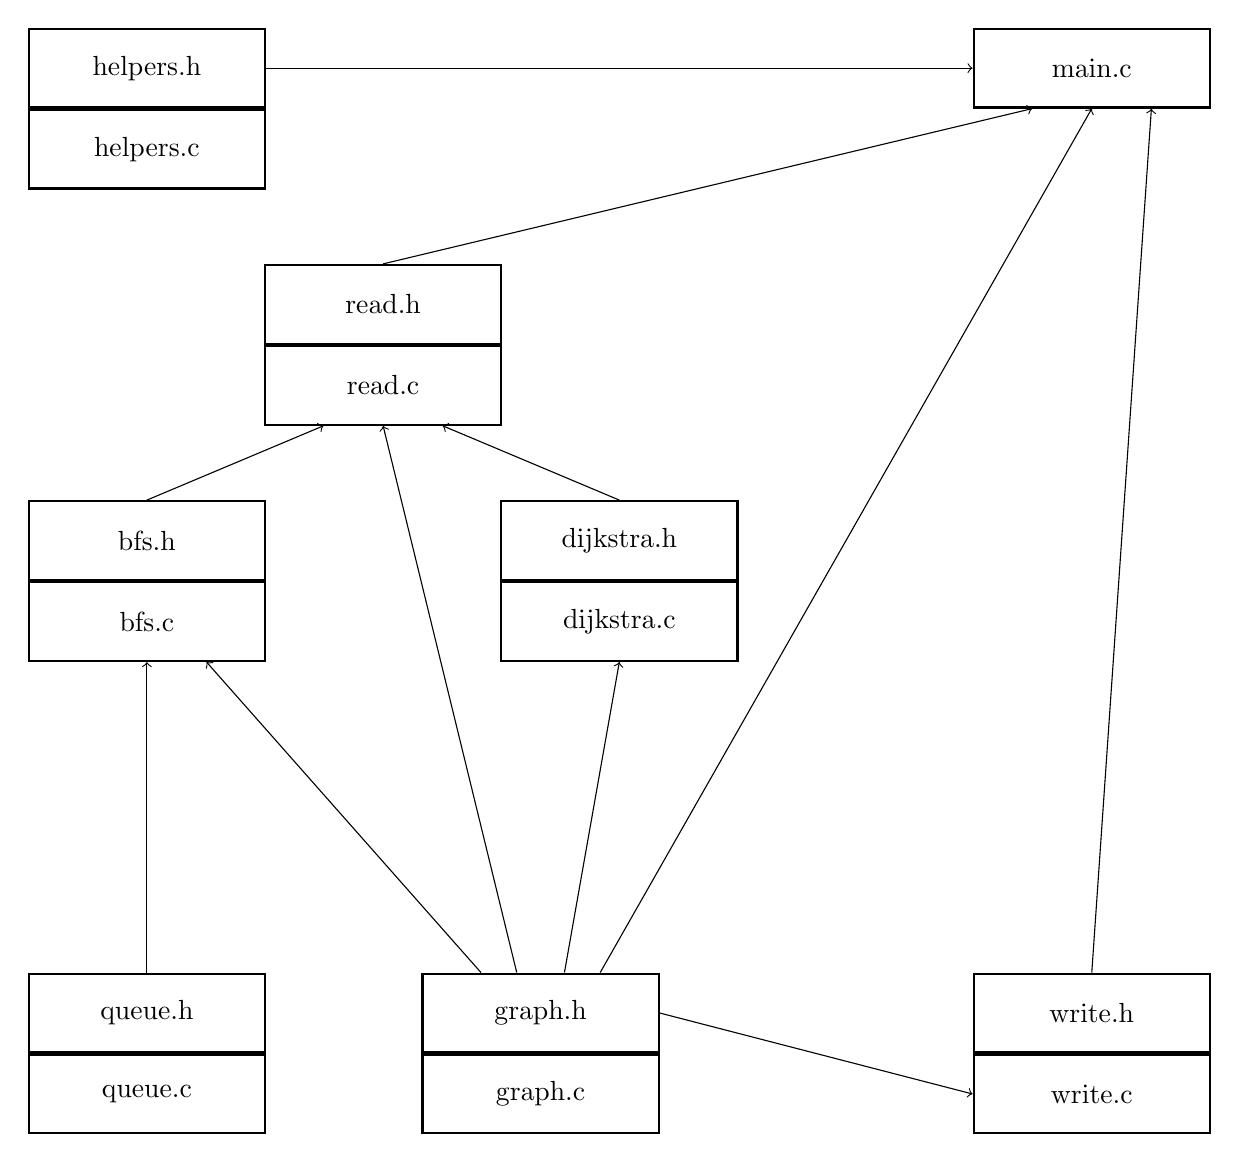
\begin{tikzpicture}
        [
            file/.style={rectangle, draw, thick, minimum width=3cm, minimum height=1cm}
        ]
        %nodes
        \node[file] at (0,0)                    (queue_h)       {queue.h};
        \node[file, below=0cm of queue_h]       (queue_c)       {queue.c};
        \node[file] at (5,0)                    (graph_h)       {graph.h};
        \node[file, below=0cm of graph_h]       (graph_c)       {graph.c};
        \node[file] at (0,6)                    (bfs_h)         {bfs.h};
        \node[file, below=0cm of bfs_h]         (bfs_c)         {bfs.c};
        \node[file] at (6,6)                    (dijkstra_h)    {dijkstra.h};
        \node[file, below=0cm of dijkstra_h]    (dijkstra_c)    {dijkstra.c};
        \node[file] at (3,9)                    (read_h)        {read.h};
        \node[file, below=0cm of read_h]        (read_c)        {read.c};
        \node[file] at (12,0)                   (write_h)       {write.h};
        \node[file, below=0cm of write_h]       (write_c)       {write.c};
        \node[file] at (0,12)                   (helpers_h)     {helpers.h};
        \node[file, below=0cm of helpers_h]     (helpers_c)     {helpers.c};
        \node[file] at (12,12)                  (main_c)        {main.c};
        %arrows
        \draw[->] (queue_h.north) -- (bfs_c.south);
        \draw[->] ($(graph_h.north west)!0.5!(graph_h.north)$) -- ($(bfs_c.south)!0.5!(bfs_c.south east)$);
        \draw[->] ($(graph_h.north west)!0.6!(graph_h.north east)$) -- (dijkstra_c.south);
        \draw[->] ($(graph_h.north west)!0.4!(graph_h.north east)$) -- (read_c.south);
        \draw[->] (graph_h.east) -- (write_c.west);
        \draw[->] ($(graph_h.north)!0.5!(graph_h.north east)$) -- (main_c.south);
        \draw[->] (bfs_h.north) -- ($(read_c.south west)!0.5!(read_c.south)$);
        \draw[->] (dijkstra_h.north) -- ($(read_c.south)!0.5!(read_c.south east)$);
        \draw[->] (write_h.north) -- ($(main_c.south)!0.5!(main_c.south east)$);
        \draw[->] (read_h.north) -- ($(main_c.south west)!0.5!(main_c.south)$);
        \draw[->] (helpers_h.east) -- (main_c.west);
    \end{tikzpicture}
    \\
    \\
    \\
    Objaśnienie:
    \\
    \\
    \begin{center}
        \begin {tikzpicture}
            [
                file/.style={rectangle, draw, thick, minimum width=2cm, minimum height=0.8cm}
            ]
            \node[file] at (0,0)                    (queue_h)       {queue.h};
            \node[file, below=0cm of queue_h]       (queue_c)       {queue.c};
            \node[file] at (4,0)                    (read_h)        {read.h};
            \node[file, below=0cm of read_h]        (read_c)        {read.c};
            \draw[->] (queue_h.east) -- (read_c.west);
        \end{tikzpicture}
    \end{center}
    Plik \verb|queue.h| jest dołączany do pliku \verb|read.c| (oraz ewentualnie do \verb|read.h|). To znaczy że w pliku \verb|read.c| (oraz ewentualnie w \verb|read.h|) znajduje się dyrektywa \verb|#include "queue.h"|.

    \newpage
    \section{Plik main.c}
    Plik źródłowy (\verb|main.c|) zawiera stałe *\_o i help oraz definicje funkcji:
    \begin{itemize}
        \item \verb|write_init|
        \item \verb|read_init|
        \item \verb|main|
    \end{itemize}
    \subsection{Stałe *\_o}
    \verb|const char* *_o[2]| (np. \verb|const char* file_o[2]|)\\
    Stałe te przechowują nazwy argumentów wywołania, gdzie pierwszym elementem jest długa (normalna) nazwa argumentu, a drugim nazwa skrócona.\\
    \subsection{Stała help}
    \verb|const char* help|\\
    Stała ta przechowuje pomoc, zawierającą instrukcję wywołania i opisy wszystkich argumentów.\\
    \subsection{Funkcja write\_init}
    \verb|int write_init(int argc, char* argv[])|\\
    Funkcja ta sprawdza argumenty wywołania dla trybu zapisu i ich wartości, a następnie wywołuje funkcję odpowiedzialną za tryb zapisu. Funkcja zwraca wartości \verb|EXIT_SUCCESS| lub \verb|EXIT_FAILURE|.\\
    \subsection{Funkcja read\_init}
    \verb|int read_init(int argc, char* argv[])|\\
    Funkcja ta sprawdza argumenty wywołania dla trybu czytania i ich wartości, a następnie wywołuje funkcję odpowiedzialną za tryb czytania. Funkcja zwraca wartości \verb|EXIT_SUCCESS| lub \verb|EXIT_FAILURE|.\\
    \subsection{Funkcja main}
    \verb|int main(int argc, char* argv[])|\\
    Funkcja ta sprawdza, który tryb został wybrany, a następnie wywołuje funkcje \verb|write_init| lub \verb|read_init| (lub wyświetla pomoc jeżeli tryb nie został wybrany). Funkcja zwraca wartości \verb|EXIT_SUCCESS| lub \verb|EXIT_FAILURE|.\\

    \newpage
    \section{Pliki write.c i .h}
    Plik źródłowy (\verb|write.c|) zawiera stałą \verb|ec_drawing_weight| oraz definicje funkcji:
    \begin{itemize}
        \item \verb|gen_graph|
        \item \verb|write|*
    \end{itemize}
    Plik nagłówkowy (\verb|write.h|) zawiera deklaracje zaznaczonych funkcji z pliku źródłowego (*).\\
    \subsection{Stała ec\_drawing\_weight}
    \verb|const int ec_drawing_weight[5]|\\
    \\
    Stała ta przechowuje informację o wagach losowania dla poszczególnych liczb krawędzi. Na przykład wartości \verb|{1,2,3,4,5}| oznaczają że wraz z liczbą krawędzi rośnie szansa na wylosowanie danej liczby krawędzi, gdyż tablica z której losowana będzie liczba krawędzi będzie wyglądać tak: \verb|{0,1,1,2,2,2,3,3,3,3,4,4,4,4,4}|.\\
    \subsection{Funkcja gen\_graph}
    \verb|graph gen_graph(int width, int height, double edge_weight_min, double edge_weight_max,|\\
    \verb|                int edge_count_min, int edge_count_max, int seed)|\\
    \\
    Funkcja ta odpowiada za wygenerowanie grafu o szerokości (ilości kolumn) \verb|width|, wysokości (ilości wierzy) \verb|height|, gdzie każdy wierzchołek będzie miał maksymalnie \verb|edge_count_max| i (w miarę możliwości) minimalnie \verb|edge_count_min| krawędzi\footnote{liczba krawedzi jest losowana; patrz "Stała ec\_drawing\_weight"}, z których każda będzie miała wagę mieszczącą się w przedziale od \verb|edge_weight_min| do \verb|edge_weight_max| włącznie. Funkcja zwraca graf.\\
    \subsection{Funkcja write}
    \verb|int write(FILE* file, int width, int height, double edge_weight_min,|\\
    \verb|          double edge_weight_max, int edge_count_min, int edge_count_max, int seed)|\\
    \\
    Funkcja ta wywołuje funkcję \verb|gen_graph| (przekazując jej jednocześnie wszystkie swoje parametry poza \verb|file|), a następnie zapisuje uzyskany graf do pliku \verb|file|. Funkcja zwraca wartości \verb|EXIT_SUCCESS| lub \verb|EXIT_FAILURE| (funkcja nie przewiduje wystąpienia błędu, więc w praktyce jest to tylko \verb|EXIT_SUCCESS|).

    \newpage
    \section{Pliki read.c i .h}
    Plik źródłowy (\verb|read.c|) zawiera definicje funkcji:
    \begin{itemize}
        \item \verb|path_fill|
        \item \verb|path_display|
        \item \verb|bfs_init|
        \item \verb|dijkstra_init|
        \item \verb|read_graph|
        \item \verb|read|*
    \end{itemize}
    Plik nagłówkowy (\verb|read.h|) zawiera deklaracje zaznaczonych funkcji z pliku źródłowego (*).\\
    \subsection{Funkcja path\_fill}
    \verb|int path_fill(d_result result, int *nv, int from, int to)|\\
    \\
    Funkcja ta odpowiada za wypełnienie tablicy \verb|nv| numerami wierzchołków, które tworzą ścieżkę od \verb|from| do \verb|to|, na podstawie tablicy poprzedników wygenerowanej przez algorytm Dijkstry i przechowywanej w strukturze \verb|result|. Funkcja zwraca ilość dodanych wierzchołków do tablicy.\\
    \subsection{Funkcja path\_display}
    \verb|void path_display(int *nv, int l)|\\
    \\
    Funkcja ta odpowiada za wyświetlenie ścieżki pomiędzy dwoma wierzchołkami przechowywanej w tablicy \verb|nv| znając jej długość \verb|l|.\\
    \subsection{Funkcja bfs\_init}
    \verb|void bfs_init(graph g)|\\
    \\
    Funkcja ta odpowiada za wywołanie algorytmu BFS i wyświetlenie komunikatu o spójności grafu \verb|g|.\\
    \subsection{Funkcja dijkstra\_init}
    \verb|void dijkstra_init(graph g, int vertex_a, int vertex_b)|\\
    \\
    Funkcja ta odpowiada za wywołanie algorytmu Dijkstry i wyświetlenie najkrótszej ścieżki pomiędzy wierzchołkami \verb|vertex_a| i \verb|vertex_b| lub najkrótszych ścieżek pomiędzy wierzchołkiem \verb|vertex_a| i pozostałymi wierzchołkami grafu \verb|g|.\\
    \subsection{Funkcja read\_graph}
    \verb|graph read_graph(FILE *f)|\\
    \\
    Funkcja ta odpowiada za odczytanie grafu z pliku \verb|f|, tworzenie struktury grafu i uzupełnienie jej przeczytanymi wierzchołkami i wagami z pliku. Funkcja zwraca stworzoną strukturę grafu.\\
    \subsection{Funkcja read}
    \verb|int read(FILE *file, int connectivity, int vertex_a, int vertex_b)|\\
    \\
    Funkcja odpowiada za zarządzanie trybem read. Przyjmuje wskaźnik na plik (bądź stdin), z którego ma być czytany graf, a także czy ma być sprawdzona jego spójność (\verb|connectivity| przyjmuje wartość 1/0) oraz numery wierzchołków, między którymi ma być wyznaczona ścieżka (gdy \verb|vertex_b| jest równy -1, wyznaczana jest ścieżka pomiędzy \verb|vertex_a| i wszystkimi wierzchołkami).

    \newpage
    \section{Pliki dijkstra.c i .h}
    Plik źródłowy (\verb|dijkstra.c|) zawiera definicje funkcji:
    \begin{itemize}
        \item \verb|result_init|*
        \item \verb|result_free|*
        \item \verb|dijkstra|*
    \end{itemize}
    Plik nagłówkowy (\verb|dijkstra.h|) poza deklaracjami zaznaczonych funkcji z pliku źródłowego (*) zawiera także deklarację struktury wyniku generowanego przez algorytm Dijkstry.\\
    \subsection{Struktura d\_result}
    \verb|typedef struct r|\\
    \verb|{|\\
    \verb|    double *d;|\\
    \verb|    int *p;|\\
    \verb|} *d_result;|\\
    \\
    Struktura przechowuje dwie tablice: \verb|d| - zawierającą całkowitą wagę dojścia do danego wierzchołka z wierzchołka początkowego oraz \verb|p| – zawierającą numery poprzedników.\\
    \subsection{Funkcja result\_init}
    \verb|d_result result_init(int n, int vertex_a, int *visited)|\\
    \\
    Funkcja ta odpowiada za zainicjalizowanie struktury typu \verb|d_result| i wypełnienie jej tablic w taki sposób jaki wymaga tego algorytm Dijkstry (tablica \verb|d| wypełniona nieskończonościami oprócz elementu o indeksie wierzchołka początkowego; tablica \verb|p| wypełniona wartościami -1). Oprócz tego uzupełnia tablicę \verb|visited| zerami. Funkcja zwraca utworzoną strukturę.\\
    \subsection{Funkcja result\_free}
    \verb|void result_free(d_result result)|\\
    \\
    Funkcja ta odpowiada za zwolnienie pamięci zarezerwowanej dla struktury \verb|result|.\\
    \subsection{Funkcja dijkstra}
    \verb|d_result dijkstra(graph graph, int vertex_a)|\\
    \\
    Funkcja ta odpowiada za wykorzystanie algorytmu Dijkstry do uzupełnienia tablic struktury typu \verb|d_result|. Funkcja zwraca utworzoną strukturę.\\

    \newpage
    \section{Pliki bfs.c i .h}
    Plik źródłowy (\verb|bfs.c|) zawiera definicje funkcji:
    \begin{itemize}
        \item \verb|bfs|*
    \end{itemize}
    Plik nagłówkowy (\verb|bfs.h|) zawiera deklaracje zaznaczonych funkcji z pliku źródłowego (*).\\
    \subsection{Funkcja bfs}
    \verb|int* bfs(graph graph, int vertex)|\\
    \\
    Funkcja ta jest implementacją algorytmu BFS (Breadth-first search) w uproszczonej wersji. Sprawdza czy w grafie \verb|graph| od wierzchołka \verb|vertex| istnieją ścieżki do wszystkich pozostałych wierzchołków. Funkcja zwraca tablicę liczb 0/1 (prawda/fałsz) o długości [ilość wierzchołków grafu], w której index oznacza numer wierzchołka a wartość wynik sprawdzenia dla wierzchołka o danym indeksie.\\

    \newpage
    \section{Pliki graph.c i .h}
    Plik źródłowy (\verb|graph.c|) zawiera definicje funkcji:
    \begin{itemize}
        \item \verb|graph_init|*
        \item \verb|graph_free|*
        \item \verb|edge_list_add|*
        \item \verb|edge_list_contains_vertex|*
        \item \verb|edge_list_length|*
    \end{itemize}
    Plik nagłówkowy (\verb|graph.h|) poza deklaracjami zaznaczonych funkcji z pliku źródłowego (*) zawiera także deklarację struktury grafu w formie listy sąsiedztwa (\verb|graph|) oraz deklarację struktury listy wierzchołków (\verb|edge_list|).\\
    \subsection{Struktura graph}
    \verb|typedef struct g|\\
    \verb|{|\\
    \verb|    int width;|\\
    \verb|    int height;|\\
    \verb|    edge_list **list;|\\
    \verb|} *graph;|\\
    \\
    Struktura przechowuje szerokość grafu (liczba kolumn) (\verb|width|), wysokość grafu (liczba wierszy) (\verb|height|) oraz tablicę list połączonych wierzchołków dla każdego wierzchołka (lista sąsiedztwa) (\verb|list|).\\
    \subsection{Struktura edge\_list}
    \verb|typedef struct e|\\
    \verb|{|\\
    \verb|    int vertex;|\\
    \verb|    double weight;|\\
    \verb|    struct e *next;|\\
    \verb|} edge_list;|\\
    \\
    Struktura przechowuje numer połączonego wierzchołka (\verb|vertex|), wagę krawędzi (\verb|weight|) oraz wskaźnik na następny element (\verb|next|) (lista jednokierunkowa).\\
    \subsection{Funkcja graph\_init}
    \verb|graph graph_init(int w, int h)|\\
    \\
    Funkcja ta odpowiada za zainicjalizowanie grafu o szerokości (ilości kolumn) \verb|w| i wysokości (ilości wierszy) \verb|h|. Funkcja zwraca graf\\
    \subsection{Funkcja graph\_free}
    \verb|void graph_free(graph g)|\\
    \\
    Funkcja ta odpowiada za zwolnienie pamięci zarezerwowanej dla grafu \verb|g|.\\
    \subsection{Funkcja edge\_list\_add}
    \verb|edge_list* edge_list_add(edge_list *l, int v, double wt)|\\
    \\
    Funkcja ta odpowiada za dodanie na koniec listy połączonych wierzchołów \verb|l| nowego wierzchołka o numerze \verb|v| i wadze krawędzi \verb|wt|. Funkcja zwraca wskaźnik na listę połączonych wierzchołków.\\
    \subsection{Funkcja edge\_list\_contains\_vertex}
    \verb|int edge_list_contains_vertex(edge_list* l, int v)|\\
    \\
    Funkcja ta odpowiada za sprawdzenie czy na liście połączonych wierzchołków \verb|l| znajduje się wierzchołek o numerze \verb|v|. Funkcja zwraca wartości 1/0 (prawda/fałsz).\\
    \subsection{Funkcja edge\_list\_contains\_vertex}
    \verb|int edge_list_length(edge_list* l)|\\
    \\
    Funkcja ta odpowiada za sprawdzenie długości listy połączonych wierzchołków \verb|l|. Funkcja zwraca długość listy.\\

    \newpage
    \section{Pliki queue.c i .h}
    Plik źródłowy (\verb|queue.c|) zawiera definicje funkcji:
    \begin{itemize}
        \item \verb|queue_enqueue|*
        \item \verb|queue_dequeue|*
    \end{itemize}
    Plik nagłówkowy (\verb|queue.h|) poza deklaracjami zaznaczonych funkcji z pliku źródłowego (*) zawiera także deklarację struktury kolejki FIFO (First in, first out) (\verb|queue|).\\
    \subsection{Struktura queue}
    \verb|typedef struct q|\\
    \verb|{|\\
    \verb|    int value;|\\
    \verb|    struct q* next;|\\
    \verb|} queue;|\\
    \\
    Struktura przechowuje wartość pojedyńczego elementu (\verb|value|) oraz wskaźnik na następny element (\verb|next|) (lista jednokierunkowa).\\
    \subsection{Funkcja queue\_enqueue}
    \verb|void queue_enqueue(queue** q, int value)|\\
    \\
    Funkcja ta odpowiada za dodanie na początku kolejki \verb|q| (listy) nowego elementu o wartości \verb|value|.\\
    \subsection{Funkcja queue\_enqueue}
    \verb|int queue_dequeue(queue** q)|\\
    \\
    Funkcja ta odpowiada za pobranie wartości elementu z końca kolejki \verb|q| (listy), usunięcie ostatniego elementu z kolejki, a następnie zwrócenie pobranej wartości.\\

    \newpage
    \section{Pliki helpers.c i .h}
    Plik źródłowy (\verb|helpers.c|) zawiera definicje funkcji:
    \begin{itemize}
        \item \verb|str_arr_get_index|*
        \item \verb|str_is_int|*
        \item \verb|str_is_double|*
    \end{itemize}
    Plik nagłówkowy (\verb|helpers.h|) zawiera deklaracje zaznaczonych funkcji z pliku źródłowego (*).\\
    \subsection{Funkcja str\_arr\_get\_index}
    \verb|int str_arr_get_index(char* element, const char* array[], int length)|\\
    \\
    Funkcja ta odpowiada za znalezienie w tablicy napisów \verb|array| o długości \verb|length| konkretnego napisu \verb|element|. Funkcja zwraca indeks tego napisu w tablicy.\\
    \subsection{Funkcja str\_is\_int}
    \verb|int str_is_int(char* string)|\\
    \\
    Funkcja ta odpowiada za sprawdzenie czy napis \verb|string| jest liczbą całkowitą (tzn. napis zawiera tylko cyfry i ewentualnie znak minus na początku). Funkcja zwraca wartości 1/0 (prawda/fałsz).\\
    \subsection{Funkcja str\_is\_double}
    \verb|int str_is_double(char* string)|\\
    \\
    Funkcja ta odpowiada za sprawdzenie czy napis \verb|string| jest liczbą rzeczywistą (tzn. napis zawiera tylko cyfry oraz ewentualnie jedną kropkę i znak minus na początku). Funkcja zwraca wartości 1/0 (prawda/fałsz).\\

    \newpage
    \section{Plik makefile}
    Plik \verb|makefile| przechowuje instrukcje kompilacji programu oraz instrukcję czyszczenia folderu (\verb|clean|) i instrukcję testu (\verb|test|).\\
    \subsection{Kompilacja (make)}
    Instrukcja kompilacji składa się z czterech etapów:
    \begin{enumerate}
        \item wygenerowania pliku zawierającego zależności\\
              (\verb|cc -MM [pliki źródłowe] > [plik zaw. zależności]|)
        \item wczytania go (\verb|-include [plik zaw. zależności]|)
        \item skompilowania programu (\verb|cc -o gridgraph [pliki .o]|)
        \item czyszczenia pokompilacyjnego (\verb|rm [pliki .o] [plik zaw. zależności]|)
    \end{enumerate}
    \subsection{Czyszczenie (make clean)}
    Instrukcja czyszczenia usuwa pliki (wywoływana jest komenda \verb|rm [pliki]|):
    \begin{itemize}
        \item plik programu
        \item pliki .o
        \item plik zawierający zależności
    \end{itemize}
    \subsection{Test (make test)}
    Instrukcja testu w pierwszej kolejności wywołuje instrukcję kompilacji, a następnie
\end{document}